\documentclass[conference,letterpaper,twocolumn]{IEEEtran}
%\usepackage[latin1]{inputenc}
%\usepackage[ansinew]{inputenc}
\usepackage[utf8]{inputenc}

\usepackage{graphicx}
\usepackage{psfrag}
\usepackage{stfloats}
%\usepackage[spanish]{babel}
\usepackage{epsfig}
\usepackage{pifont}
\usepackage{amssymb}
\usepackage{fixltx2e}
\usepackage{amsmath}
\usepackage{rotate}
\usepackage{anysize}
%\usepackage{rotating}
%\usepackage{fancybox}
\usepackage{float}
\usepackage{fancybox}
\usepackage{subfig}

\newcommand{\pig}[1]{\mbox{\boldmath ${#1}$}	}

\newtheorem{Theod}{{\bf Definici\'on}}

\setlength{\oddsidemargin}{5mm}
\setlength{\evensidemargin}{5mm}
\setlength{\topmargin}{4mm}
\setlength{\textwidth}{15cm}
\setlength{\columnsep}{5mm}
\setlength{\textheight}{24cm}

\begin{document}

\title{Double bounded bi-parameter homotopy applied to bipolar/diode circuit simulation}

\author{\authorblockN\centerline{{H\'ector V\'azquez-Leal, Roberto Casta\~neda-Sheissa and Uriel Filobello-Niño }}
\authorblockA{University of Veracruz\\
Electronic Instrumentation School\\
Xalapa, Veracruz, M\'exico\\
Email: hvazquez@uv.mx}
\and
\authorblockN{\centerline{Arturo Sarmiento-Reyes and Luis Hern\'andez-Mart\'{\i}nez}}
\authorblockA{National Institute for Astrophysics, Optics and Electronics\\
Electronics Department\\
Email: jarocho@inaoep.mx}
}

\maketitle

\begin{abstract}

This works presents a biparametric homotopy with automated stop criterion. Its principal characteristic is to posses symmetry axis, double bounding solution line, random initial and final points and a method to establish the biparametric function. Besides, this method will be exemplified by using a circuit with multiple operating points. Last, the effects of the parametric function over the homotopy path will be discussed.
\end{abstract}
 
\section{Introduction} 
Solution to non-linear equation systems is needed for several areas of physiscs, particularly, in electronics the solution to non-linear algebraic equation systems (NAES) allows to figure out the approximate behaviour of integrated circuits, before they are fabricated, allowing the designers to optimize/redesign their circuits in order to lower costs. The most employed method to solve NAES is the Newton-Raphson (NR) method, which has quadratic convergence \cite{homo_ogrodzki,cont_quasi}. Therefore, homotopy methods have been proposed because they have better convergence than the NR method. Likewise, the complexity of circuits have been continuously increasing, this translates in a greater probability of an unnoticed existence of multiple operating points \cite{netwth_4q}; these situation can be solved using homotopy methods since they are capable to locate multiple solutions over one path, contrary to the NR method, it just can locate one solution per simulation.

\section{Homotopy}
Equilibrium equation for any circuit can be formulated using the modified nodal analysis (MNA) \cite{mnaxx} as initial step, it is defined as:

\begin{equation}
{f}({x})={0} \qquad \text{where} \qquad f:\in \mathfrak{R}^n \to  \mathfrak{R}^n,
\label{fx}
\end{equation}

here $x$ represents the electrical variables of the circuit, and $n$ the number of nodes plus the number of non-NA compatible elements.

Homotopy methods are based on the fact that solutions are connect by a curve, called "solution curve". To obtain this curve one additional parameter is added to the original equation system, it will help to obtain the following augmented equation:

{\small
\begin{equation}
{H}({f}({x}),\lambda )={0}  \quad \text{where} \quad {H}: \in \mathfrak{R}^n \times  \mathfrak{R} \to \mathfrak{R}^n,
\label{homotopia}
\end{equation}}

where $(H)$ represents the homotopy function, $\lambda$ the continuation parameter, and ${f}({x})$ the original equation to be solved.

Thus, the original problem becomes a numerical continuation problem \cite{homo_richter}; here the continuation variable it the homotopy parameter $\lambda$. Therefore, ${H}({f}({x}),0)={G}({x})$, where ${G}: \in \mathfrak{R}^n \to  \mathfrak{R}^n$ is an smooth map which has one trivial solution and ${H}({f}({x}),1)={f}({x})$, meaning that at $\lambda=1$ the solution of ${f}({x})$ is located.

A homotopy example is given by:

\begin{equation}
{H}({f}({x}),\lambda ) =
{f}({x})-(1-\lambda ){f}({x}_{0}) = 0
\label{hexampl}
\end{equation}

When $\lambda =0$, one known solution is obtained (a priori) at ${x}_{0}$, usually a trivial solution and at $\lambda =1$ is located the solution for ${f}({x})=0$. 

\section{Multiparameter Homotopy}
Multiparametric homotopy adds more than one homotopy parameter to the equilibrium equation \cite{homo_DWolfMulti}. Essentially, it has a similar behaviour to the uniparametric homotopy, because it has one trivial solution when the homotopy parameters has value of zero and the solution for $f(x)$ is located when the homotopy parameters reach the value of one. The multiparametric homotopy can be represented as:

\begin{equation}
{H}({f}({x}),\lambda_1,\lambda_2,...,\lambda_k)=0,
\end{equation}

where $\lambda_1,\lambda_2,...\lambda_k\in[0,1]$, $k$ is the number of homotopy parameters, and $x$ represents the nodal voltages and currents of the non-NA compatible elements.

On one hand, the multiparametric homtopies \cite{homo_DWolfMulti} have been proposed to avoid fork bifurcations, singularities, among other problems that can be found on the homotopy paths. On the other hand, multiparametric homotopy applied to circuits can be interpreted as the non-linear circuit deformation in a simplified circuit with trivial solution, such that when homotopy parameters are swept, the simplified circuit is transformed until it coincides with the original non-linear circuit. Therefore, this type of homotopy produces a soft convergence to the final solution. That circuital transformation is of broad interest since it is possible to created custom homotopies to solve circuits characterized by specific non-linearities like circuits composed of devices like: BJT/MOS transistors, memristors, nanotubes, among others. Likewise, it is possible to apply multiparameter homotopies to the models of devices in order to linearize the circuit right at the beginning of the homotopy path; softly returning its original state (nonlinear) as the homotopy parameters reach the value of 1.

\section{Double bounded biparameter homotopy}
It is possible to formulate a multiparametric homotopy with stop criterion using the the double bounded polynomial homotopy \cite{xxx}, its formulation is:

\begin{equation}
{
\begin{array}{l}
{H}({f}({x}),\lambda )=QP - W {f}({x})^2
\end{array}}
\label{homotopiaP}
\end{equation}

where $Q=\lambda(\lambda-a)$,  $P=(x-x_i)(x-x_f)$, $W=C(\lambda_1-a/2)^2$, $\lambda_1$ is the homotopy parameter, $a$ is a constant that represents the separation between solution lines $\lambda_1=0$ and $\lambda_1=1$, $x_i$ is the initial point, $x_f$ the final point, and $C$ an arbitrary constant. A second homotopy parameter is added; now, the homotopy is formulated as:

\begin{equation}
{\small
\begin{array}{l}
{H}({f}({x}),\lambda_1, \lambda_2 )=QP - W {f}({x},\lambda_2)^2
\end{array}}
\label{homotopiaPx1}
\end{equation}

here $Q=\lambda_1(\lambda_1-a)$, ${f}({x},\lambda_2)$ represents the insert of the second homotopy parameter  $\lambda_2$ within the equilibrium equation ${f}({x})$, $P=(x-x_i)(x-x_f)$, and $W=C(\lambda_1-a/2)^2$.

The MNA method establishes that a stimuli vector exists, it contains the independent current sources, nonlinear voltage and current sources contributions. The new variables (currents) appear in the equilibrium equation as additional unknowns.

\begin{equation}
\left[ \begin{array}{c}
\text{ \it GMNA}
\end{array} \right]
\left[ \begin{array}{c}
{v} \\
{i} \\
\end{array} \right]
=
\left[ \begin{array}{c}
{i_{est}}
\end{array} \right]
\end{equation}

where GMNA represents a matrix containing the contributions of linear conductances and the branch relationships of the non-NA compatible elements, ${v}$ represents the nodal voltages of the circuit, ${i}$ represents the currents of the non-NA compatible elements, and ${i_{est}}$ represents the contributions to the stimulus vector from all the independent current sources, voltage drops in the independent voltage sources, and the contributions of the nonlinear voltage and current sources.

In a circuit containing bipolar transistors, the Eber-Moll model contains diodes whose most simple model is a nonlinear current source that depends exponentially on the voltage drop in the diode. Therefore, the contribution of the nonlinear current source to the equation will be placed directly in the stimulus vector $i_{est}$.

The addition of the homotopy parameter into the equilibrium equation should be done in such a way that the homotopy path follows a path as soft as possible; this can be achieved multiplying $\lambda$ by the nonlinear  branch stimulus vector of the components in the circuit and the power supplies. This is done to suppress nonlinearities and energy sources of the circuit just at $\lambda_2=0$. So, the multiparametric homotopy function proposed in this work is defined as:

\begin{equation}
{\small
\begin{array}{l}
H(f(x),\lambda_1, \lambda_2 )=QP - Wf(x,\lambda_2i_{est})^2
\end{array}}
\label{homotopiaPx3}
\end{equation}

here $Q=\lambda_1(\lambda_1-a)$, $P=(x-x_i)(x-x_f)$ y $W=C(\lambda_1-a/2)^2$. Besides, the
multiparametric homotopy can be expressed in general way as (using $a=1$):

{\small
\begin{displaymath}
{H}(\cdot)= \left\{\begin{array}{rl}
f(x^*)=0 & \textrm{for  $\lambda_1=1, \lambda_2=1$ and $x=x^*$}\\
P=0 & \textrm{for $\lambda_1=0.5$ and $\lambda_2=0$}\\
f(x^*)=0 & \textrm{for $\lambda_1=0, \lambda_2=1$ and $x=x^*$}
\end{array}\right.
\end{displaymath}
}

where $P=(x-x_i)(x-x_f)$ and the homotopy function depends of ${H}({f}({x}),\lambda_1,\lambda_2{i_{est}})$.

The homotopy parameter $\lambda_2$ does not interfere directly with the homotopy formulation, nevertheless, $\lambda_2$ is added to the equilibrium equation $f(x)$, therefore, the remaining of the properties for the multiparametric homotopy coincides witht the homotopy reported in \cite{xxx1}, those are: symmetrical branches, symmetry axis, initial and final points for the homotopy path, and stop criterion.

In summary, the double bounded homotopy has the following characteristics:

\begin{itemize}
\item Simmetry axi. It is an imaginary axis, divides the homotopy path into two symmetrical branches, right at $\lambda_{sym}=a/2$. This is the axis where the initial and final points of the homotopy path are located.
\item Initial point ($\lambda_i$). For $\lambda_1=0.5$ and $\lambda_2=0$ the solution of $H^{-1}(0)$ is known ($x_i$). 
\item Symmetrical branch 1. For $\lambda_1=1$ and $\lambda_2=1$, ${H}({f}({x}),1,1)={f}({x})$. Means that at $\lambda_1=1$ and $\lambda_2=1$ all the solutions for ${f}({x})$ are located.
\item Symmetrical branch 2. For $\lambda_1=0$ and $\lambda_2=1$, ${H}({f}({x}),0,1 )={f}({x})$. This means that at $\lambda_1=0$ and $\lambda_2=1$ all the solutions for ${f}({x})$ are located.
\item Final point  ($\lambda_f$). For $\lambda_1=0.5$ and $\lambda_2=0$ the solution of $H^{-1}(0)$ is known ($x_f$). 
\end{itemize}

The homotopy function $(H)$ is a function of $n+2$ variables with $n$ equations; $n$ equals to the total number of nodes plus the non-NA compatible elements. Hence, it is necessary one extra equation to use the conventional tracing techniques for homotopy paths \cite{homo_allgower}. The equation is a function of $\lambda_1$ and $\lambda_2$ which will be called multiparamtric function $M(\lambda_1,\lambda_2)=0$. Such equation must cross by ${\lambda}_i=[\lambda_1,\lambda_2]=[0.5,0]$ and by ${\lambda}_s=[\lambda_1,\lambda_2]=[1,1]$. ${\lambda}_i$ is the point where the solution of the circuit is trivial and ${\lambda}_s$ is the point where the solution for ${H}$ is exactly the desired solution for the equilibrium equation ${f}({x}_s)=0$. The excursion of $\lambda_1$ starts at 0.5 because the symmetry axis has been established at $\lambda_{sym}=0.5$. Nevertheless, intermediate points of the homotopy path $\lambda_1-\lambda_2$ are not defined and they play an important role on the softness of the entire homotopy path. Therefore, the following equation is proposed as the multiparametric function:

{
\begin{equation}
\begin{array}{c}
M(\lambda_1,\lambda_2)=-\lambda_{{1}}+\\ { \left( \lambda_{{2}}+{\frac {B \left( - 1+A \right) }
{AB+ 1- 2A}} \right) \over  \left( -{\frac { \left( - 1+ 2\,
A- B \right) \lambda_{{2}}}{AB+ 1- 2A}}+ 2\,{\frac {B
 \left( - 1+A \right) }{AB+ 1- 2A}} \right) }
\end{array}
\label{homotopiaPx4}
\end{equation}
}

where $[\lambda_1,\lambda_2]=[A,B]$ is the point where the curve cross the curve of the function $M(\lambda_1,\lambda_2)$, as shown in Fig. \ref{curvasl}(a). The value range for $A$ and $B$ is $[0,1]$.

\begin{figure}[hbtp]
\psfrag{o}{$\lambda$}
\centering
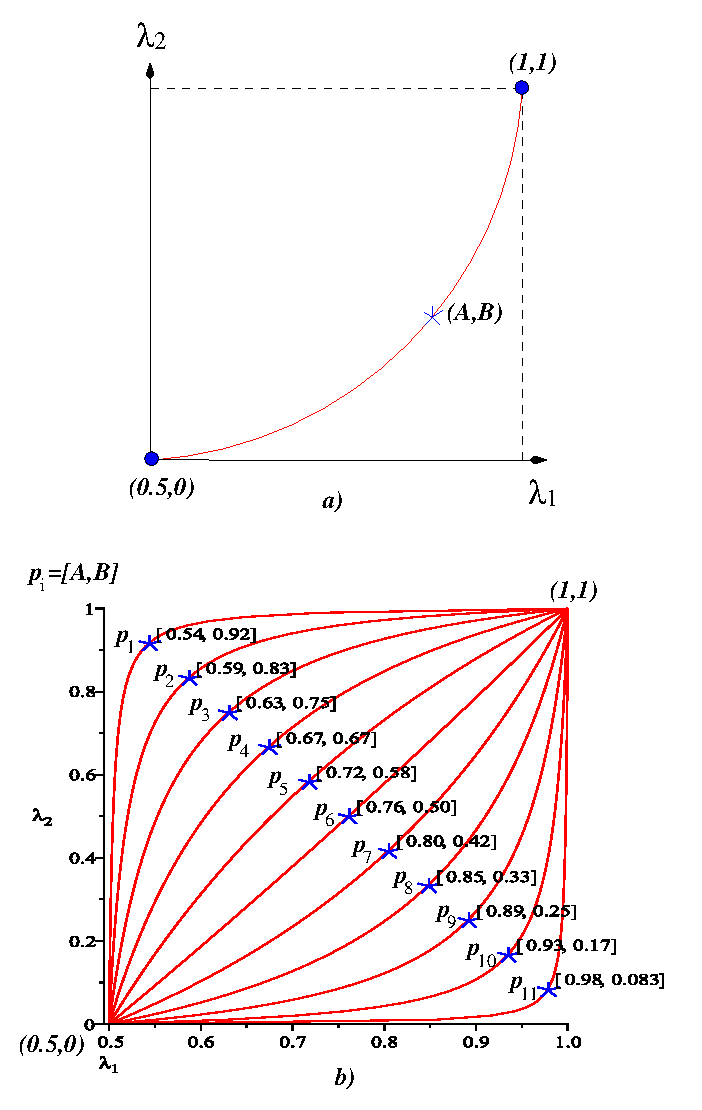
\includegraphics[scale=0.6]{fig/curvasl.eps}
\caption{Path of $M(\lambda_1,\lambda_2)=0$ for different points $p=[A,B]$.}
\label{curvasl}
\end{figure}

\section{Study case: circuit with bipolar transistors and a diode}

A circuit with bipolar transistors and a diode was reported in \cite{homo_yamamura}. The circuit was solved using the modified fixed point Homotopy. This circuit has three operating points. The Ebers-Moll model is used for all the transistors; the equation for the model is given by:

\begin{displaymath}
\left[ \begin{array}{c}
i_{D_E} \\
i_{D_C}
\end{array}\right] =
\left[ \begin{array}{cc} 1  & \alpha_R \\
\alpha_F & 1 \\
\end{array}\right] \left[ \begin{array}{c}
10^{-9}(e^{(40v_{be})} - 1) \\
10^{-9}(e^{(40v_{bc})} - 1)
\end{array}\right]
\end{displaymath}

As for the diode, the model is:

\begin{displaymath}
i_d=10^{-9}(e^{40u} - 1)
\end{displaymath}

\begin{figure}[hbtp]
\centerline{
\epsfxsize=75mm
\epsffile{yamamura/diotran.eps}
}
\caption{Circuit with bipolar transistors and a diode.}
\label{yamamuracircuito}
\end{figure}

First, the equilibrium equation is formulated using the modified nodal analysis obtaining a system containing 14 equations and 14 variables. The circuit is shown in Fig. \ref{yamamuracircuito}.

Now, double bounded homotopy is applied to solve the circuit; the Homotopy formulation is expressed as follows:

\begin{displaymath}
{\small
\begin{array}{r}
H_1(\cdot)=Q(v_1-13)(v_1+13)+ W f_1^2=0\\
H_2(\cdot)=Q(v_2-13)(v_2+13)+ W f_2^2=0\\
\vdots \qquad \\
H_{13}(\cdot)=Q(v_{13}-13)(v_{13}+13)+ W f_{13}^2=0\\
H_{14}(\cdot)=Q(I_E-13)(I_E+13)+ W f_{14}^2=0\\
M(\lambda_1,\lambda_2)=0
\end{array}}
\end{displaymath}


where $Q=\lambda_1(\lambda_1-1)$, $W=C(\lambda_1-0.5)^2 $, the value of the constant value is $C=1$, the bounding lines are $[\lambda_1,\lambda_2]=[0,1]$ and $[\lambda_1,\lambda_2]=[1,1]$, nodal equations $f$ depend of $(v_1,v_2,\hdots,v_{13},I_E,\lambda_2i_{est})$.

The circuit is simulated with a conventional tracing technique like the ones shown in  \cite{homo_allgower,homo_iberchip03}. In order to show the effects of specifically selecting a parametric function $M(\lambda_1,\lambda_2)=0$, four particular cases were chosen.

\begin{enumerate}
\item $M_1$ path associated to point $p_1$. This path is an extreme case of parametric function, it is characterized by distorting first the $\lambda_1$ parameter from about zero until one and subsequently distort $\lambda_2$ from about zero until one (see Fig. \ref{curvasl}(b)).
\item $M_6$ path associated to point $p_6$. This path represents the case where homotopy parameters keep an approximately  linear aspect ratio (Fig. \ref{curvasl}(b)).
\item $M_{11}$ path associated to point $p_{11}$. This path is an extreme case of parametric function, which is characterized by qualitatively distort, first, $\lambda_2$ parameter from about zero until 1 and subsequently distort $\lambda_1$ from about zero until 1 (see Fig. \ref{curvasl}(b)).
\item $M_{12}$ path. In Fig. \ref{yamaie}(g) a case of polynomial homotopy function level 3 is shown.
\end{enumerate}

Table \ref{yamamuracircuitosoluc} summarize the results of tracing all four homotopy paths, each one with a different multiparametric function. Besides, the four paths share the same initial point. Then, found results are shown:

\begin{itemize}
\item All four paths showed double bounding ($\lambda_1=0$ y $\lambda_1=1$ ) and symmetry axis $\lambda_{sym}=0.5$.
\item The corresponding symmetrical branch was traced successfully [$\lambda_1=1,\lambda_2=1$].
\item For every case all three operating points were located (see Table \ref{yamamuracircuitosoluc1}).
\item The number of turning points (TP) is eleven for all four paths.
\item The final point for paths $M_1$ and $M_{11}$ is the same. This implies that extreme paths may be similar no matter which parameter is swept first ($\lambda_1$ or $\lambda_2$).
\item The final point for the linear path $M_{6}$ differs from the other paths ($M_1$, $M_11$, and $M_{12}$).This result implies that it is possible affect the homotopy path depending on the selection made for the parametric function $M$.
\item A polynomial parametric function ($M_{12}$) was implemented as:

{\small
\begin{displaymath}
\begin{array}{c}
M(\lambda_1,\lambda_2)=-\lambda_2+ 98.09523810\lambda_1^3- \\ 221\lambda_1^2+ 161.8333333\lambda_1-37.92857143
\end{array}
\end{displaymath}
}

The multiparametric function $M_{12}$ is shown in Fig. \ref{yamaie}(g) and its corresponding homotopy path in Fig. \ref{yamaie}(i) and \ref{yamaie}(j). In this case, the total number of iterations (Iter) were lower than the iterations reached using parametric functions: $M_1$, $M_6$, and $M_{11}$,  even the final point of the path is different in the final points to the rest of the paths. Therefore, the selection of the parametric function plays an important role on the performance of the double bounded biparametric homotopy.
\end{itemize}

The same number of solutions and turning points but different number of iterations means that the four paths have similar aspects as shown in Fig. \ref{yamaie}. Nevertheless, the different number of iterations suggests that the four paths cross through the same equilibrium equation folds, with slight differences on the exact location of turning points and the value of the radius of curvature changes both to the return points and the bounce points on solutions (see Fig. \ref{yamaie}). Last, $M_6$ path has higher number of iterations and a different final point (compared to $M_1$, $M_{11}$, and $M_{12}$) meaning that it is possible to affect the homotopy path with an appropriate $M$ selection. In the presented study case fewer number of iterations were achieved in the most nonlinear parametric function ($M_{12}$), therefore, there are nonlinear functions $M$ able to optimize the homotopy path.

In \cite{homo_MOS} a multiparametric homotopy was proposed, which locates just one operating point per simulation, does not have an automated stop criterion, symmetry or solution lines that bound the path, so, in this sense the proposed homotopy in this work shows certain advantages. Also, in \cite{homo_MOS} circuit simulations containing up to 8489 transistors were shown. Although the study case shown here was done with bipolar transistors/diodes, it is possible to generalize the described technique to circuits containing MOS transistors, since the model for such transistors contains a nonlinear current source, which is considered in the proposed method.

\begin{figure*}[hbtp]
\centerline{
\epsfxsize=105mm
\epsffile{fig/yamamu.eps}
}
\caption{Homotopy path for $v_2-\lambda_1$}
\label{yamaie}
\end{figure*}

\begin{table*}[htbp]
{\small
\center{
\hspace{-4mm}
\begin{tabular}{||c|c|c|c|c|c|c|c|c|c|c|c|c|c|c|c|c||}
\hline\hline
Points & Iter & TP &$v_1$ & $v_2$ & $v_3$ & $v_4$ & $v_5$ & $v_6$ & $v_7$ & $v_8$ & $v_9$ & $v_{10}$& $v_{11}$ & $v_{12}$ & $v_{13}$ & $i_E$  \\ \hline
$x_i$ & - & - &+13 & +13& +13& -13& +13& +13& +13& +13& +13& +13& +13& +13& -13& -13  \\ \hline
$x_f(M_1)$ & 16669 & 11&+13& +13& +13& -13& +13& +13& +13& +13 & +13& +13&+13&+13&-13&+13   \\ \hline
$x_f(M_6)$ & 17063 &11 & +13 & -13 & +13 &-13& +13&  +13& +13& +13& +13& +13& +13& +13& -13& +13     \\ \hline
$x_f(M_{11})$ & 16508 &11 &+13& +13 & +13& -13& +13& +13& +13&+13& +13& +13& +13& +13& -13 &+13  \\ \hline 
$x_f(M_{12})$ & 16112 &11 &+13& +13 & -13& -13& +13& +13& +13&+13& +13& +13& +13& +13& -13 &+13  \\ \hline \hline
\end{tabular}
}
}
\caption{Extreme points for three homotopy paths, considering $\lambda_1=0.5$ and $\lambda_2=0$.}
\label{yamamuracircuitosoluc}
\end{table*}


\begin{table*}[hbtp]
{\small
\center{
\hspace{-4mm}
\begin{tabular}{||c|c|c|c|c|c|c|c|c|c|c|c|c|c|c||}
\hline\hline
Sol & $v_1$ & $v_2$ & $v_3$ & $v_4$ & $v_5$ & $v_6$ & $v_7$ & $v_8$ & $v_9$ & $v_{10}$& $v_{11}$ & $v_{12}$ & $v_{13}$ & $i_E$ \\ \hline
$S_1$ &  12 & 5.995 & 0.085 &0.368 &0.712 &0.436 &0.390 &0.699 &11.635 &0.4e-5 &0.039 &0.039 &0.321 &-0.0089 \\ \hline
$S_2$ & 12 & 0.883 & 0.278 &0.590 &0.631 &0.812 &0.315 &1.074 &11.647 &0.4e-5 &0.039 &0.039 &0.321 &-0.0100 \\ \hline
$S_3$ & 12 & 0.405 & 0.366 &0.685 &0.349 &6.796 &0.070 &7.038 &11.839 &0.4e-5 &0.039 &0.039 &0.321 &-0.0085 \\ \hline \hline
\end{tabular}
}
}
\caption{Three Operating points (solutions) found at $\lambda_1=1$ and $\lambda_2=1$}
\label{yamamuracircuitosoluc1}
\end{table*}


\section{Conclusion}

This work has shown that it is possible to create a double bounded biparametrical homotopy, which showed a double solution line, symmetry axis, initial and final points for the path. Also, it is possible to affect the homotopy path selecting different parametric functions; likewise, different homotopy simulations for the same circuit, selecting the same initial point and different parametric functions, resulting that for the most nonlinear function showed the lowest number of iterations to complete the tracing of a symmetrical branch. Therefore, the selection of the parametric function can affect the homotopy path. Nevertheless, study is required that includes tests with bigger circuits, and other types of parametric functions, to establish selection criteria for the parametric function that generates the shortest homotopy path.

\bibliographystyle{amsplain}
\bibliography{n4hletter2}

\end{document}
